\documentclass[20pt,]{extarticle}
\usepackage[margin=0.6in]{geometry}
\pagenumbering{gobble}
\usepackage{lmodern}
\usepackage{amssymb,amsmath}
\usepackage{ifxetex,ifluatex}
\usepackage{fixltx2e} % provides \textsubscript
\ifnum 0\ifxetex 1\fi\ifluatex 1\fi=0 % if pdftex
  \usepackage[T1]{fontenc}
  \usepackage[utf8]{inputenc}
\else % if luatex or xelatex
  \ifxetex
    \usepackage{mathspec}
  \else
    \usepackage{fontspec}
  \fi
  \defaultfontfeatures{Ligatures=TeX,Scale=MatchLowercase}
\fi
% use upquote if available, for straight quotes in verbatim environments
\IfFileExists{upquote.sty}{\usepackage{upquote}}{}
% use microtype if available
\IfFileExists{microtype.sty}{%
\usepackage{microtype}
\UseMicrotypeSet[protrusion]{basicmath} % disable protrusion for tt fonts
}{}
\usepackage{hyperref}
\PassOptionsToPackage{usenames,dvipsnames}{color} % color is loaded by hyperref
\hypersetup{unicode=true,
            pdftitle={Self-Replicating Functions},
            pdfauthor={Tyler Neylon},
            colorlinks=true,
            linkcolor=black,
            citecolor=Blue,
            urlcolor=Blue,
            breaklinks=true}
\urlstyle{same}  % don't use monospace font for urls
\usepackage{graphicx,grffile}
\makeatletter
\def\maxwidth{\ifdim\Gin@nat@width>\linewidth\linewidth\else\Gin@nat@width\fi}
\def\maxheight{\ifdim\Gin@nat@height>\textheight\textheight\else\Gin@nat@height\fi}
\makeatother
% Scale images if necessary, so that they will not overflow the page
% margins by default, and it is still possible to overwrite the defaults
% using explicit options in \includegraphics[width, height, ...]{}
\setkeys{Gin}{width=\maxwidth,height=\maxheight,keepaspectratio}
\IfFileExists{parskip.sty}{%
\usepackage{parskip}
}{% else
\setlength{\parindent}{0pt}
\setlength{\parskip}{6pt plus 2pt minus 1pt}
}
\setlength{\emergencystretch}{3em}  % prevent overfull lines
\providecommand{\tightlist}{%
  \setlength{\itemsep}{0pt}\setlength{\parskip}{0pt}}
\setcounter{secnumdepth}{5}
% Redefines (sub)paragraphs to behave more like sections
\ifx\paragraph\undefined\else
\let\oldparagraph\paragraph
\renewcommand{\paragraph}[1]{\oldparagraph{#1}\mbox{}}
\fi
\ifx\subparagraph\undefined\else
\let\oldsubparagraph\subparagraph
\renewcommand{\subparagraph}[1]{\oldsubparagraph{#1}\mbox{}}
\fi
\usepackage{subfig}
\AtBeginDocument{%
\renewcommand*\figurename{Figure}
\renewcommand*\tablename{Table}
}
\AtBeginDocument{%
\renewcommand*\listfigurename{List of Figures}
\renewcommand*\listtablename{List of Tables}
}
\usepackage{float}
\floatstyle{ruled}
\makeatletter
\@ifundefined{c@chapter}{\newfloat{codelisting}{h}{lop}}{\newfloat{codelisting}{h}{lop}[chapter]}
\makeatother
\floatname{codelisting}{Listing}
\newcommand*\listoflistings{\listof{codelisting}{List of Listings}}

\title{Self-Replicating Functions}
\author{Tyler Neylon}
\date{204.2016}

% Begin custom, non-pandoc commands.

\newcommand{\latexonlyrule}{\rule}
\newenvironment{densearray}{\begin{array}{rcl}}{\end{array}}
\newcommand{\class}[1]{}
\newcommand{\Rule}[3]{}
\newcommand{\optquad}{\quad}
\newcommand{\smallscrneg}{}
\newcommand{\smallscr}[1]{}
\newcommand{\bigscr}[1]{#1}
\newcommand{\smallscrskip}[1]{}

% End custom, non-pandoc commands.

\begin{document}
\maketitle

\newcommand{\R}{\mathbb{R}}
\newcommand{\eqnset}[1]{\left.\mbox{$#1$}\;\;\right\rbrace\class{postbrace}{ }}
\providecommand{\optquad}{\class{optquad}{}}
\providecommand{\smallscrneg}{\class{smallscrneg}{ }}
\providecommand{\bigscr}[1]{\class{bigscr}{#1}}
\providecommand{\smallscr}[1]{\class{smallscr}{#1}}
\providecommand{\smallscrskip}[1]{\class{smallscrskip}{\hskip #1}}

These are notes I'm creating for myself as I explore functions \(f\)
that can be written as a sum \(f = g_1 + g_2\) where \(g_1\) and \(g_2\)
are the same up to symmetry, and both \(g_1\) and \(g_2\) strongly
resemble shifts of the original function \(f\). When a function \(f\)
has these properties, I informally call it a \emph{self-replicating
function}.

\begin{figure}
\centering
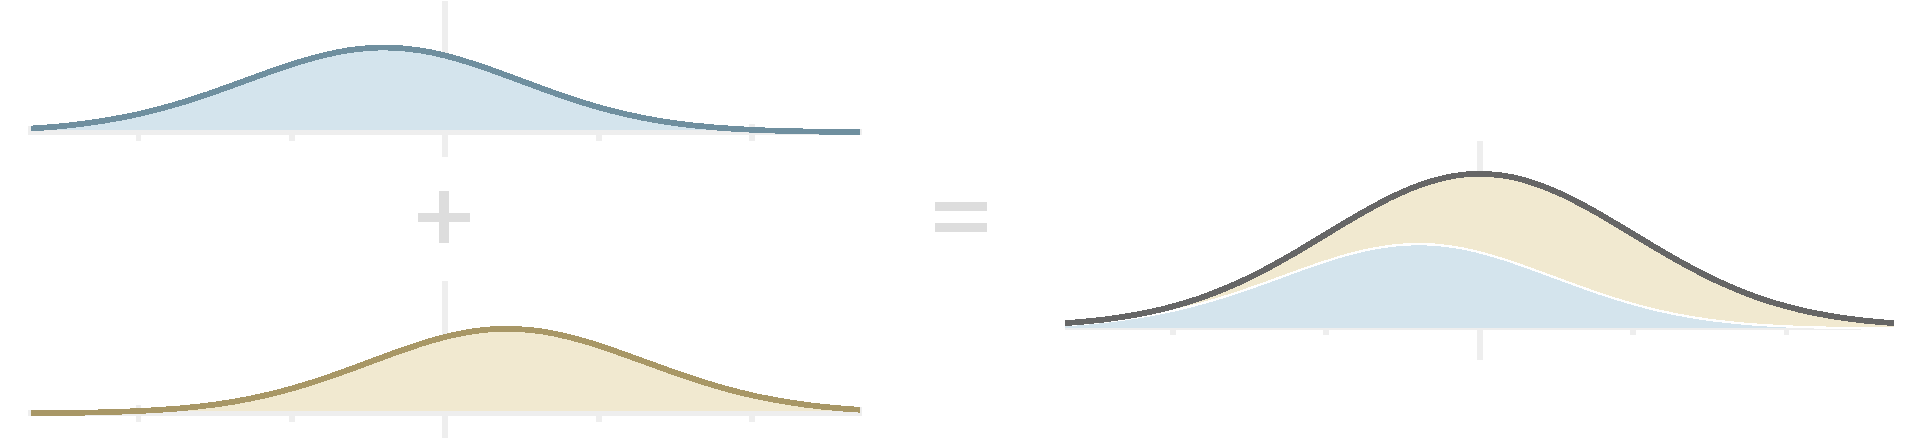
\includegraphics{images/pdfs/added_normals4.pdf}
\caption{As an example of a self-replicating function, the normal curve
can be expressed as the sum of two normal-like curves that are
reflections of each other.}\label{fig:added_normals}
\end{figure}

Like the word \emph{fractal}, this term is not rigorously defined --- in
particular, it depends on the ambiguous notion of ``strong resemblance''
--- although I plan to investigate more precise requirements below.

\section{Motivation}\label{motivation}

I became interested in self-replicating functions by working on
algorithms to procedurally generate 3d models of natural-looking trees.
When algorithmically making trees, it makes sense to start from the idea
of an \href{https://en.wikipedia.org/wiki/L-system}{\emph{L-system}},
which can be visualized as a kind of fractal in which a trunk forks into
branches that themselves fork into smaller subranches, this process
repeating infinitely.

I noticed that tree-like \emph{L}-systems can have a large amount of
``branch overlap'' concentrated around a central area of their apparent
surface. For example, consider the two images in
figure~\ref{fig:ellsystem}. On the left is a standard \emph{L}-system
along with a histogram showing the density of leaf points along the
edge. Intuitively, the leaf points are dense even toward the extreme
angles of the tree's top. However, the density increases continuously
toward the center.

We could think of each leaf point as doing a certain amount of work by
covering some area along the top of the \emph{L}-system. Each subtree is
so oblivious to its other subtrees that they overlap heavily, and the
central leaf points end up being highly redundant. To illustrate this
redundancy, the right-hand figure shows the exact same \emph{L}-system
with essentially half of the tree removed --- yet the shape formed by
the leaf points is only slightly changed.

\begin{figure}
\centering
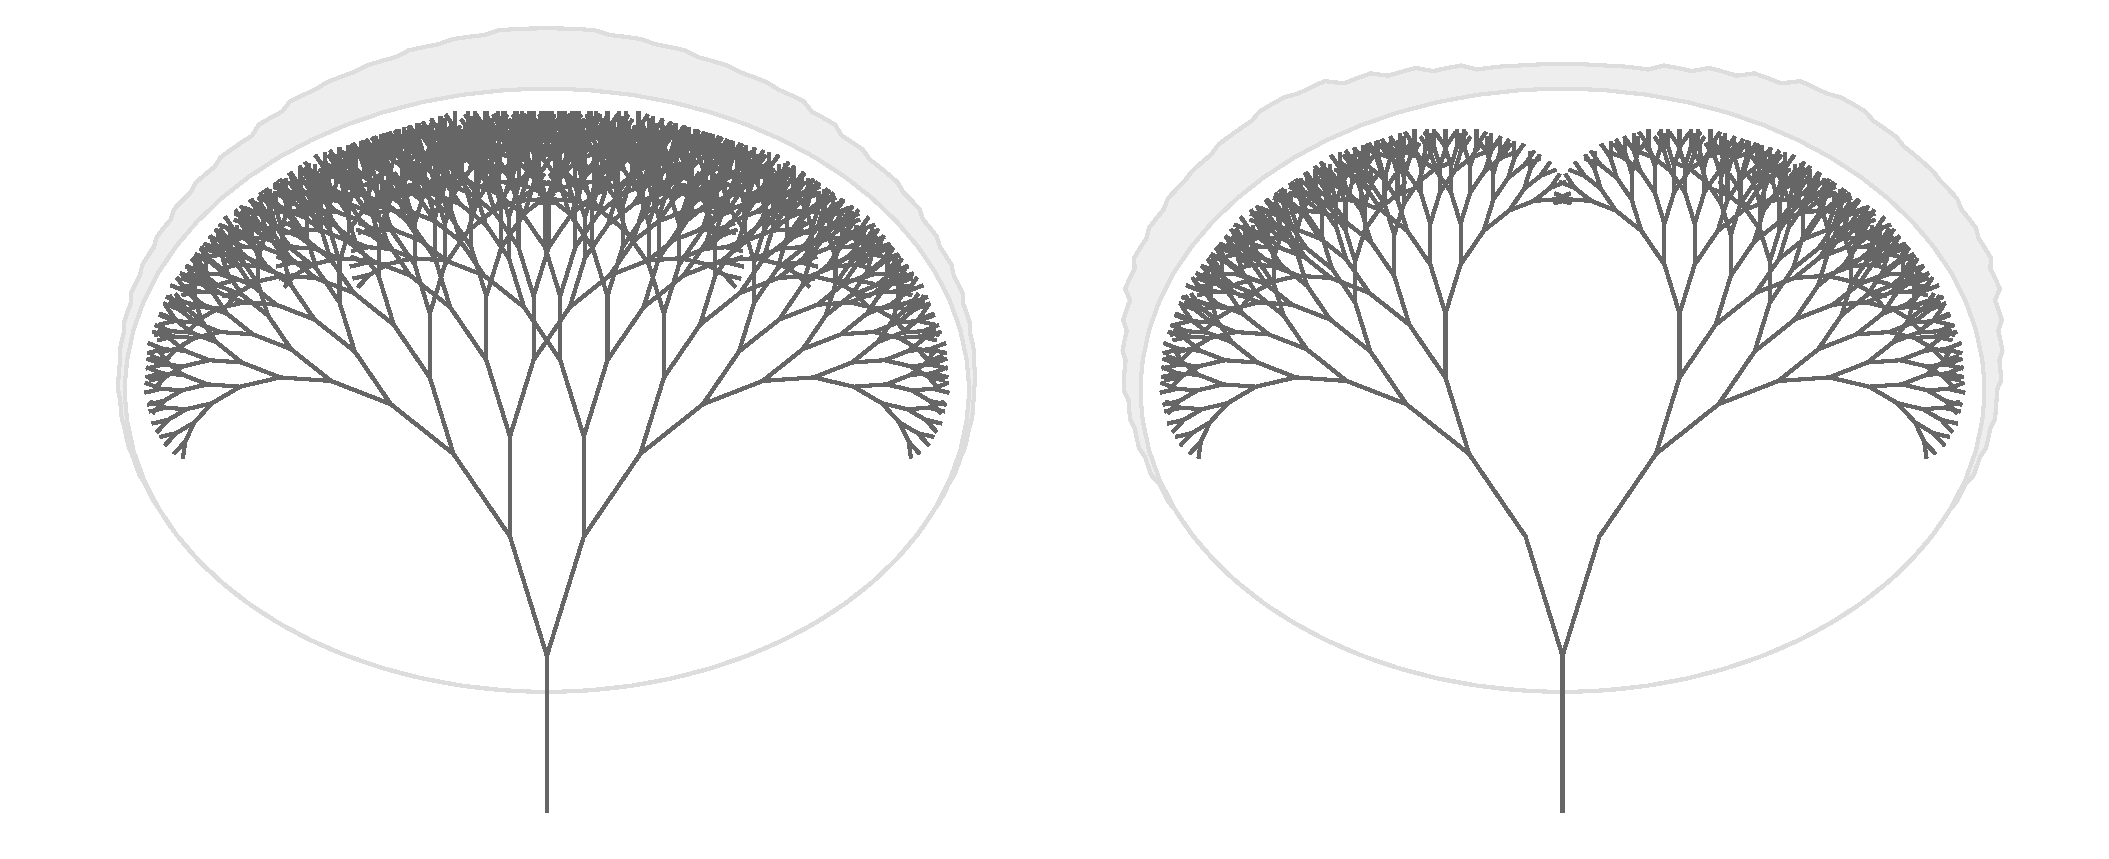
\includegraphics{images/pdfs/ellsystem2.pdf}
\caption{Left: An \emph{L}-system; Right: the same system with two large
subtrees removed. In both cases, a histogram of leaf point density is
provided around an outer ellipse.}\label{fig:ellsystem}
\end{figure}

One approach to smoothing out the distribution of leaf points would be
to compromise the fractal-like nature of the system by choosing each
line direction based on where it is within the fractal, rather than
simply by making each branching point a smaller version of its parent.
The line directions can be chosen so that the set of points at a fixed
distance from the trunk point form a set of equidistant angles from a
central point. The result is an extremely regular edge, as seen in
figure~\ref{fig:well_dist}.

\begin{figure}
\centering
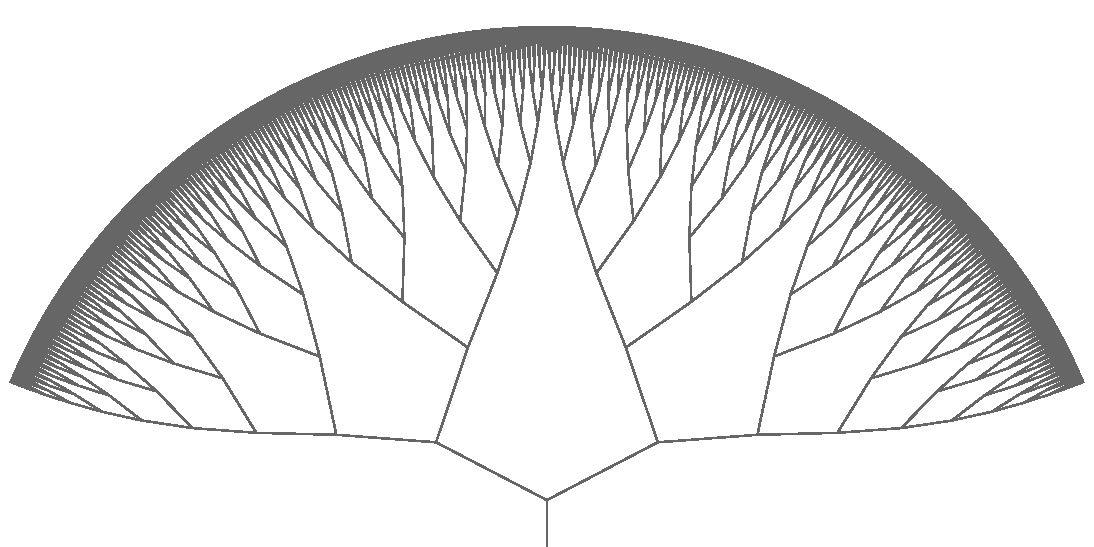
\includegraphics{images/pdfs/well_distributed_ell_like_system.pdf}
\caption{A \emph{L}-like system in which line directions are chosen to
maximize the regularity of leaf point
distribution.}\label{fig:well_dist}
\end{figure}

This is ideally efficient in that each leaf point is equally important
in forming the shape of the system. However, this system is defined in
terms of the path to each point. Is it possible to design a system so
that the overall distribution of leaf points is fairly even, yet each
subtree's shape is independent of its position within the full tree?

If this goal were achieved, we would necessarily have a leaf point
distribution which was the sum of two smaller versions of itself.
Intuitively, the leaf-point distribution of any \emph{L}-system is
already a self-replication function because, if its two main subtrees
have distribution functions \(g_1\) and \(g_2\), then the full tree has
distribution function \(f = g_1 + g_2\). I have to say
\emph{intuitively} here because I haven't formally defined the
leaf-point distribution of an \emph{L}-system.

Thus, \emph{L}-systems naturally coincide with self-replicating
functions. Although there are probably self-replicating functions which
do not correspond with \emph{L}-systems, I nonetheless find it
interesting to independently explore the world of self-replicating
functions.

\section{Simple cases}\label{simple-cases}

Technically, any polynomial can be seen as a kind of self-replicating
function. For example, if \(f(x) = x^2\),

\[\begin{densearray}
  g_1(x) & = & (x + 1)^2 - 1 = x^2 + 2x, \optquad \text{and} \\
  g_2(x) & = & (x - 1)^2 - 1 = x^2 - 2x, \\
\end{densearray}\]

then \(f = g_1 + g_2\), and each \(g_i\) is a shift of the original
function \(f\). In general, if \(f(x) = ax^n + O(x^{n-1})\) then we can
choose \(g_i(x) = a(x\pm 1)^n + O(x^{n-1})\) so that \(f = g_1 + g_2\),
and each \(g_i\) has

\[ \lim_{x\to\pm\infty}\frac{g_i(x)}{f(x)} = 1,\]

which is good enough for me to subjectively say that they strongly
resemble shifts of \(f\).

However, the original motivation for self-replicating functions is based
on distribution functions, so the rest of this note focuses on functions
\(f\) for which \(\lim_{x\to\pm\infty}f(x) = 0\).

Another simple approach would be to set \(g_1 = g_2 = \frac{1}{2}f\) for
any function \(f\). This is not very interesting, and the word
\emph{shift} in the informal definition of a self-replicating function
is intended to defeat this trivial case. That is, each \(g_i\) is
expected to be similar to a translation of \(f\), such as \(f(x-1)\) or
\(f(x+1)\).

\subsection{Indicator functions}\label{indicator-functions}

The next function I'll describe is simple and meets all of the
requirements so far. An \emph{indicator function} is a function taking
on only the value 0 or 1; it's also sometimes referred to as a
\emph{characteristic function}. If \(f\) is an indicator function, then
you can think of those \(x\) with \(f(x) = 1\) as belonging to the
subset of the domain which is \emph{indicated} by the function. It's
handy to use the following bracket notation of Knuth and others: given
any boolean predicate \(P(x)\), let \([P(x)]\) denote the value 1 when
\(P(x)\) is true, and false otherwise (Knuth 1998).

Given a half-open interval \([a, b)\), define \(I_{[a, b)}\) to be the
function \([x\in[a, b)]\). The following equation shows how such
indicator functions can be considered simple self-replicating functions:
\(I_{[0, 2)} = I_{[0, 1)} + I_{[1, 2)}\).

\begin{figure}
\centering
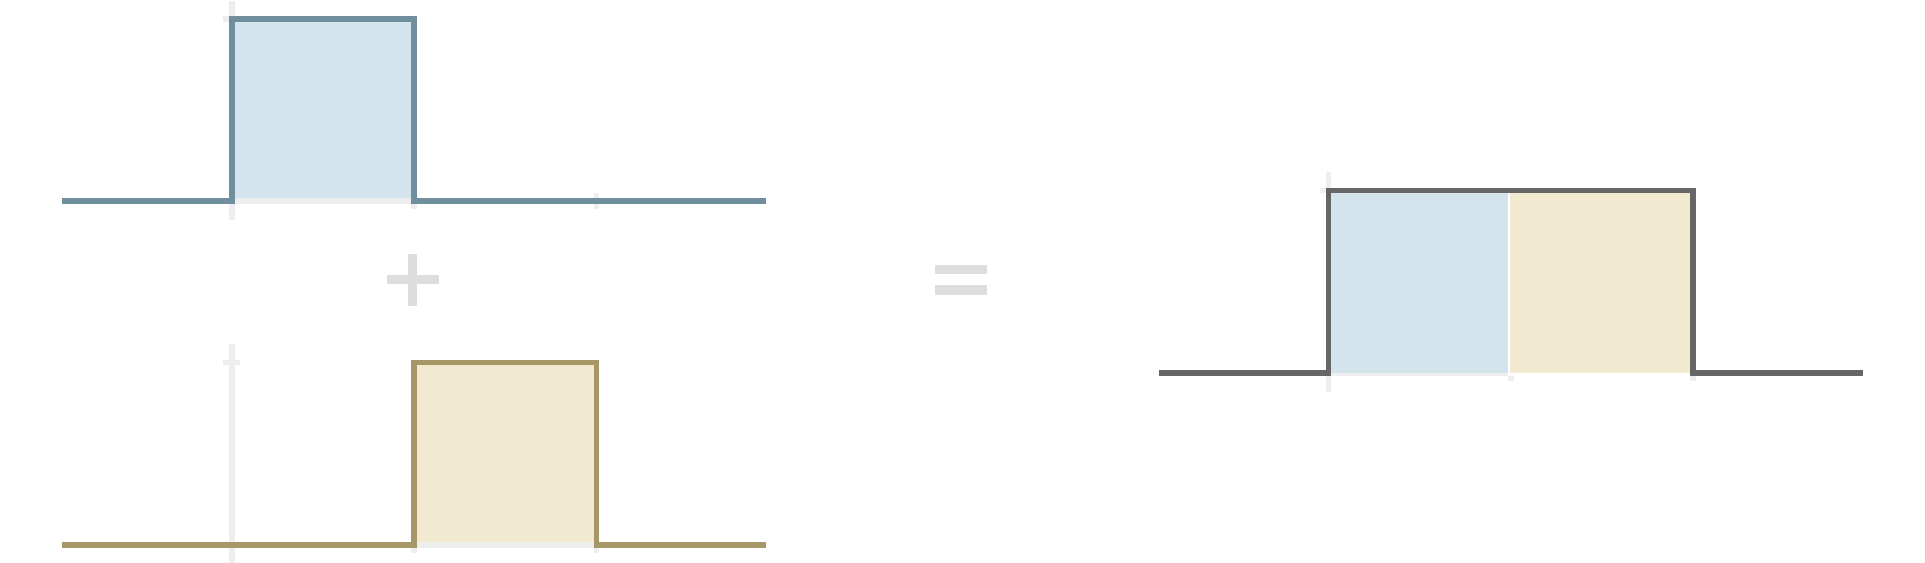
\includegraphics{images/pdfs/added_intervals6.pdf}
\caption{Visual representation of the addition of indicator functions of
intervals.}\label{fig:added_intervals}
\end{figure}

In order to match the equation \(f = g_1 + g_2\), emphasizing the
similarity between the \(g_i\)'s and \(f\), we can set
\(f = I_{[0, 2)}\), \(g_1 = f(2x) = I_{[0, 1)}\), and
\(g_2 = f(2(x - 1)) = I_{[1, 2)}\).

\subsection{Ramp functions}\label{sec:ramp_functions}

Things get more interesting when \(g_1(x) g_2(x) \ne 0\) for some \(x\).
To this end, define the \emph{ramp function} for values \(a,b,c,d\) with
\(a < b < c < d\) via

\[ J_{a,b,c,d} = \begin{cases}
\frac{x - a}{b - a} & \text{if } x \in [a, b), \\
1 & \text{if } x \in [b, c), \\
\frac{d - x}{d - c} & \text{if } x \in [c, d), \text{and} \\
0 & \text{otherwise.} \\
\end{cases}\]

Then \(J_{0,1,4,5} = J_{0,1,2,3} + J_{2,3,4,5}\), as illustrated in
figure~\ref{fig:ramp_fns}.

\begin{figure}
\centering
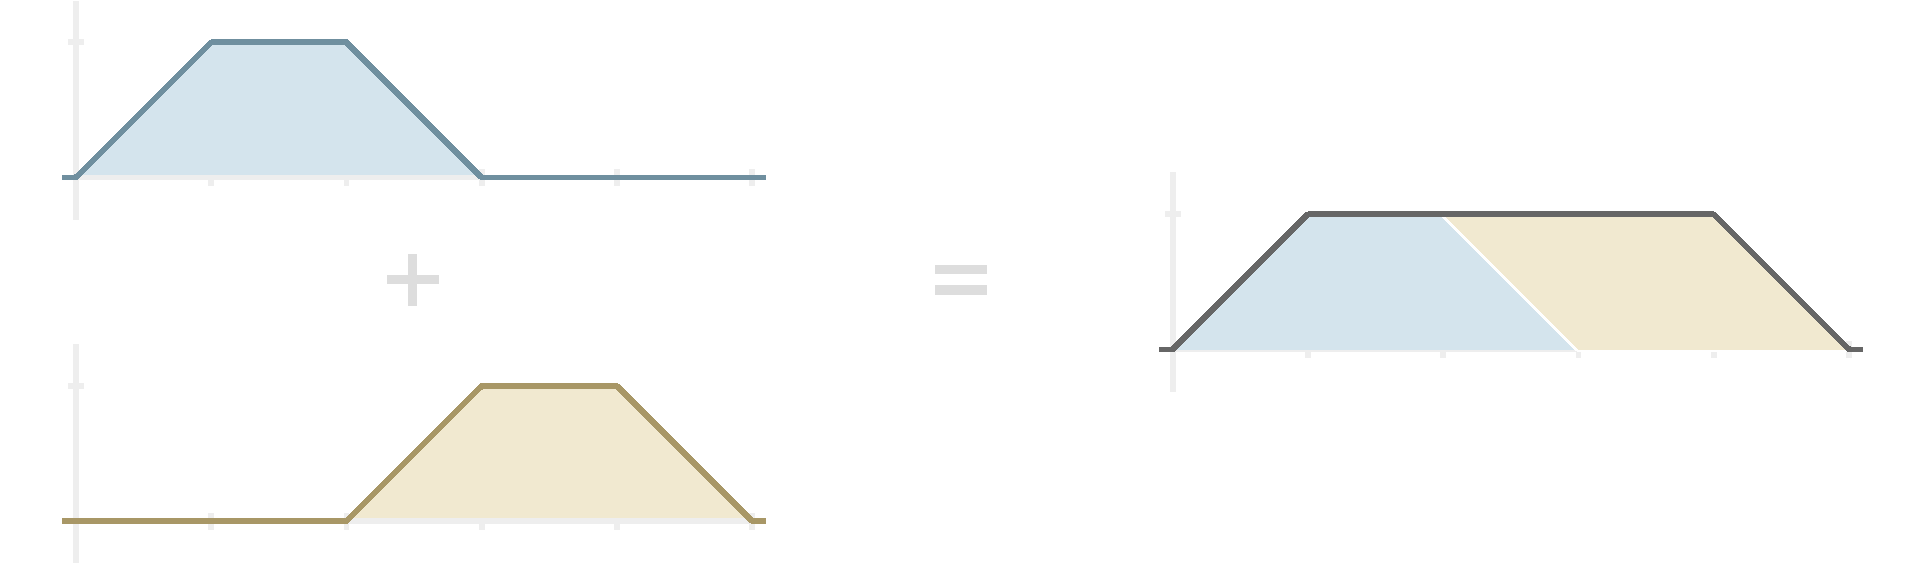
\includegraphics{images/pdfs/ramp_fns3.pdf}
\caption{Visual addition of two ramp functions to form
another.}\label{fig:ramp_fns}
\end{figure}

The ramp function example gives me four ideas for further study:

\begin{enumerate}
\def\labelenumi{\arabic{enumi}.}
\tightlist
\item
  The addends and the sum cannot be expressed as linearly related; that
  is, there is no linear function \(\ell(x)\) so that
  \(J_{0, 1, 2, 3}(\ell(x)) = J_{0, 1, 4, 5}(x)\). Contrast this with
  the interval functions where \(I_{[0, 1)}(x / 2) = I_{[0, 2)}\). This
  raises the questions: Which self-replicating functions allow for this
  linear-relation restriction? Is there a slight modification of ramp
  functions which meets this linear-relation restriction?
\item
  The ramp functions are piece-wise linear, but that linearity is not
  really the key to their being self-replicating. Rather, the key is
  that the left ramp and right ramp sum to 1, which matches the middle
  height of the functions. Which more general self-replicating functions
  can be constructed using this idea?
\item
  What happens if we treat the sum \(f = g_1 + g_2\) as part of a
  sequence? Thinking of \emph{L} and \emph{R} for \emph{left} and
  \emph{right}, let \(f^{(0)}_L = J_{0, 1, 2, 3}\), and
  \(f^{(i)}_R = f^{(i)}_L(x-2)\) for \(i \ge 0\). Thinking of \emph{S}
  for \emph{sum}, define \(f^{(i+1)}_S = f^{(i)}_L + f^{(i)}_R\) for
  \(i \ge 1\). If \(f^{(i)}_L\) is positive on \((0, b)\), then
  \(f^{(i)}_R\) is positive on \((2, b + 2)\), so \(f^{(i+1)}_S\) is
  positive on \((0, b + 2)\). Set
  \(f^{(i+1)}_L = f^{(i+1)}_S(x (b + 2) / b)\) so that we maintain the
  region on which the left function is positive. In this way, we get a
  sequence of functions. What is the limiting behavior? Can we attempt
  to extend the sequence backwards? Can we say anything in general about
  the limiting behavior of a class of starting functions \(f^{(0)}_L\)?
\item
  For the current ramp functions, the middle section is flat with value
  1, while the edges sum to 1. Can we do something more interesting
  where the edges sum to a non-constant value? I can imagine this
  leading to a discontinuous function. Is there a way to do this where
  the functions are continuous, or at least continuous almost
  everywhere? Can we describe a general class of self-replicating
  functions which are not continuous, such as the indicator function of
  the Cantor dust?
\end{enumerate}

Some of these questions will be answered below.

\subsection{Nonlinear ramps}\label{sec:nonlinear_ramps}

Other curves that sum to 1 could easily take the place of the left and
right edges of the ramp function. For example, the left and right ramps
could be replaced by curves with the shapes of \(x^2\) and \(1-x^2\) on
\(x\in [0, 1]\), as illustrated in figure~\ref{fig:nonlinear_ramps}.

\begin{figure}
\centering
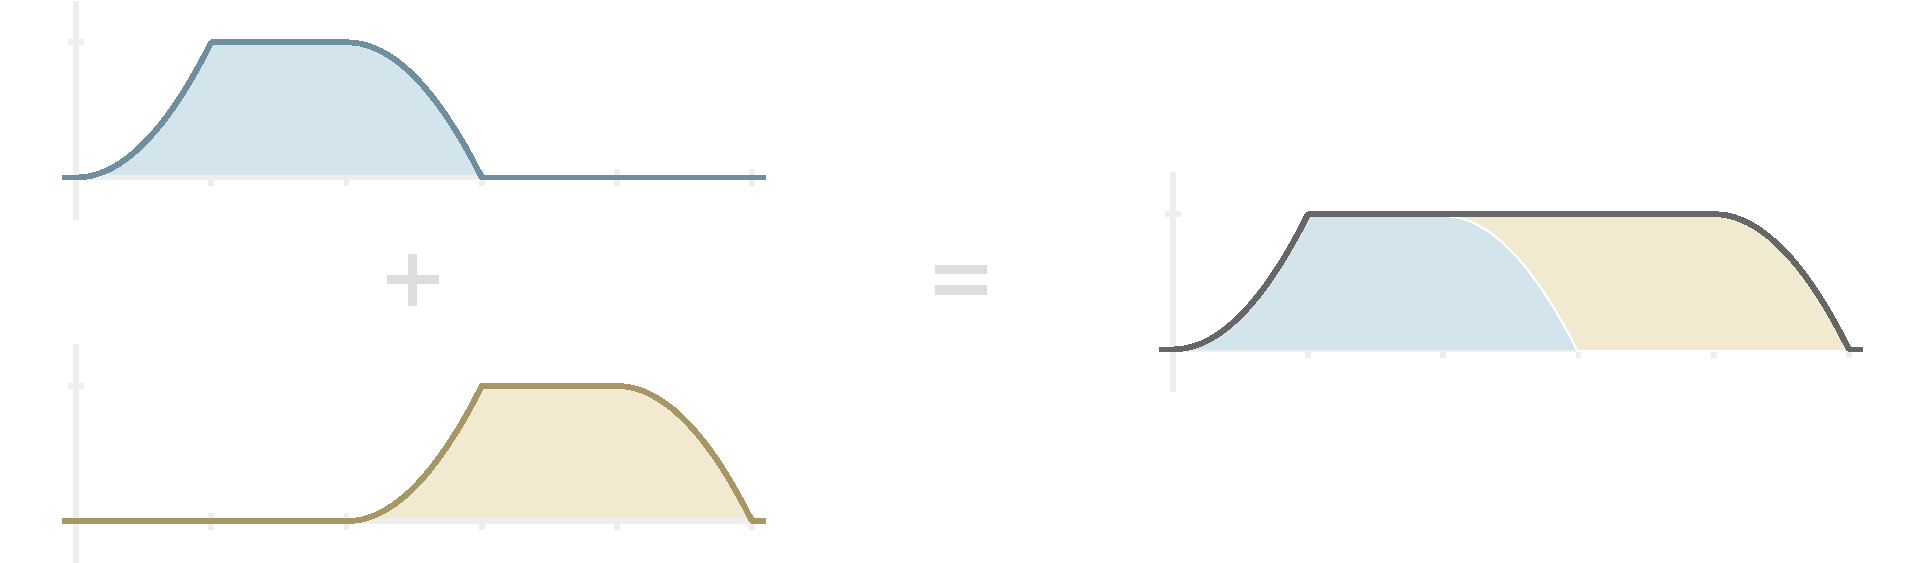
\includegraphics{images/pdfs/nonlinear_ramps2.pdf}
\caption{An example of nonlinear ramp functions using \(x^2\) on
\(x\in [0, 1]\) to determine the edge
shapes.}\label{fig:nonlinear_ramps}
\end{figure}

Given any function \(f:[0,1]\to [0,1]\), the generalized ramp function
is

\[ K_{a,b,c,d} = \begin{cases}
f\big(\frac{x - a}{b - a}\big) & \text{if } x \in [a, b), \\
1 & \text{if } x \in [b, c), \\
1 - f\big(\frac{x - c}{d - c}\big) & \text{if } x \in [c, d), \\
0 & \text{otherwise.} \\
\end{cases}\]

If any function can be written as \(K_{a,b,c,d}\) for some value of
\(f\), I'll call it a \(K-\)\emph{function}. This form is general enough
to include interval functions --- for example, by using \(f(x) = 0\)
---~and to include the previous ramp function \(J(x)\) by setting
\(f(x)=x\).

The versatility of the \(K-\)functions shows that we can produce
self-replicating functions that are highly discontinuous, such as by
setting \(f(x)\) to be the indicator function of a set with many border
elements. Even among continuous functions, we can produce
self-replicating functions which avoid being ``mostly monotonic.'' In
particular, I'll say that a function \(f:\R\to\R\) is \emph{peak
monotonic} iff there is a point \(x\) such that
\(a < b < x \Rightarrow f(a) \le f(b)\) and
\(x < c < d \Rightarrow f(c) \ge f(d)\). The indicator function of an
interval and the ramp function are both peak monotonic, while the
example \(K-\)functions in figure~\ref{fig:other_ramps} are not.

\begin{figure}
\centering
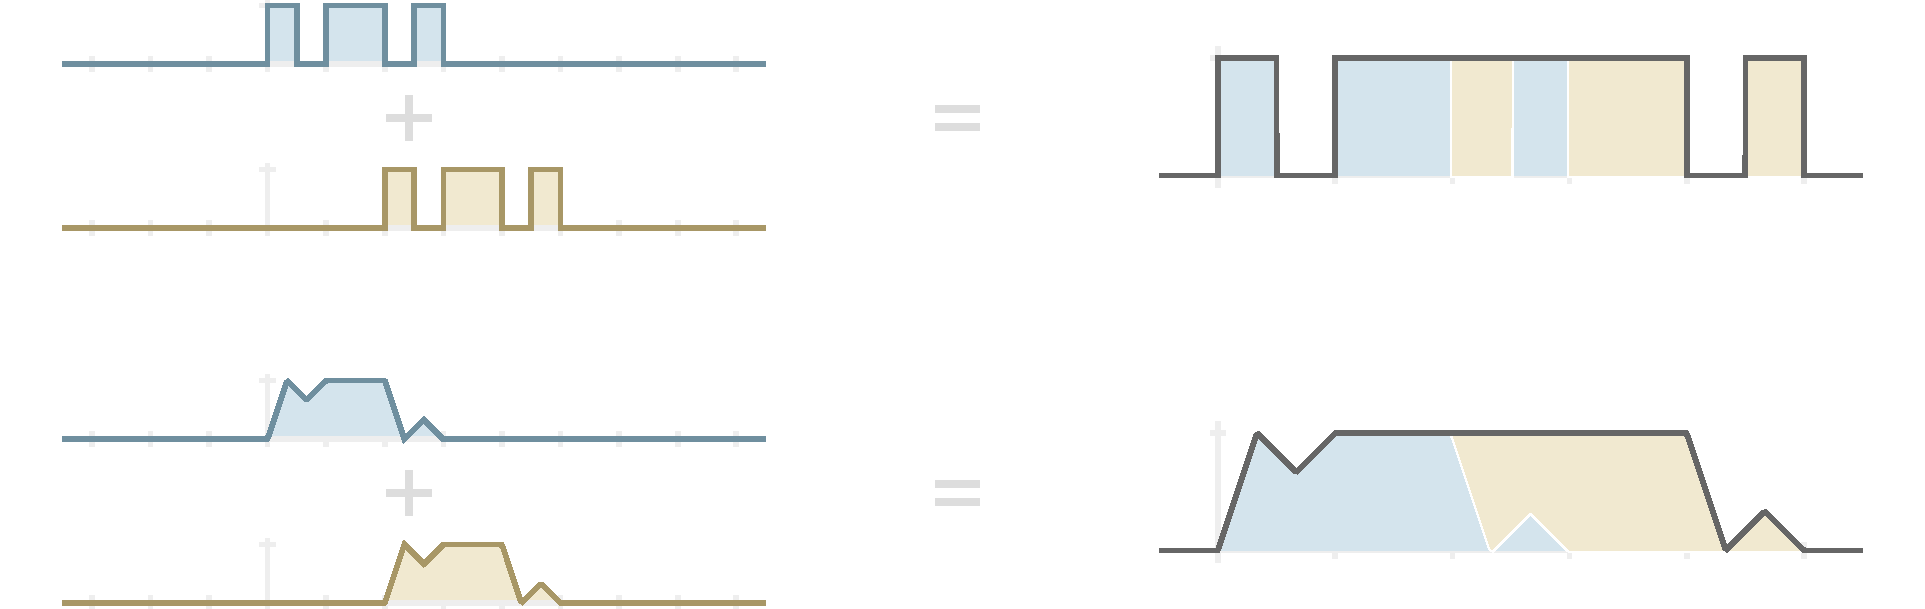
\includegraphics{images/pdfs/other_ramps2.pdf}
\caption{Example \(K-\)functions: on the top is a function more
discontinuous than the indicator function of an interval; on the bottom
is a continuous but non-peak-monotonic function.}\label{fig:other_ramps}
\end{figure}

\subsection{Non-plateau functions}\label{non-plateau-functions}

The ramp functions \(K_{a,b,c,d}\) all have the constant value 1 on the
middle interval \([b, c]\). This requires the ramps on intervals
\([a, b]\) and \([c, d]\) to sum to 1. In this section, I'll consider
what can happen if we relax this condition. I'll informally call these
\emph{non-plateau functions}.

It will be useful to propose one possible formalization of a
self-replicating function before exploring non-plateau functions.

\subsubsection{A formal definition for self-replicating
functions}\label{a-formal-definition-for-self-replicating-functions}

I think the term \emph{self-replicating function} is best left as an
intuitive, non-rigorous concept because there seem to be a wide variety
of instances that are best studied via their own particular flavors of a
formal definition. A number of other terms used to discuss mathematics
are similarly unformalized or context-specific: consider \emph{fractal},
\emph{symmetry}, or \emph{closure} as examples. Nonetheless, many
self-replicating functions meet the conditions of the definition I'll
present next.

Call a function \(f\) \emph{exactly self-replicating} iff there exist
continuous bijections \(s\), \(t_1\), and \(t_2\) such that \(s\) is not
the identity function and

\begin{equation}\eqnset{\begin{densearray}
  f_L(x)&=&f(x), \\
  f_R(x)&=&f(s(x)), \\
  f_S(x)&=&f_L(x) + f_R(x), \text{and} \\
  f_L(x)&=&t_2(f_S(t_1(x))).
\end{densearray}}\label{eq:exact_defn}\end{equation}

The \emph{L}, \emph{R}, and \emph{S} subscripts are meant to hint that
these functions act as the \emph{left} addend, \emph{right} addend, and
the \emph{sum}; the \(s\) function suggests a \emph{shift}, while the
\(t_1\) and \(t_2\) functions suggest a \emph{transformation}. The last
equation in (\ref{eq:exact_defn}) captures the similarity relationship
between the addend \(f = f_L\) and the sum \(f_S = f_L + f_R\).

\textbf{Example} The ramp functions given in §\ref{sec:ramp_functions}
and §\ref{sec:nonlinear_ramps}, viewed as \(K-\)functions, all adhere to
the general form

\[K_{0,1,2,3} + K_{2,3,4,5} = K_{0,1,4,5}.\]

In this case, \(f(x) = f_L(x) = K_{0,1,2,3}\) and
\(f_R(x) = K_{2,3,4,5} = f(x-2)\). We can satisfy all of the equations
of (\ref{eq:exact_defn}) by using these functions:

\begin{equation}\eqnset{\begin{densearray}
t_1(x) & = &
\begin{cases}
  x              &   x \le 1,       \\
  3x - 2         &   1 < x < 2,   \\
  x + 2          &   x \ge 2; \\
\end{cases}\\
t_2(x) & = & x; \text{ and} \\
s(x)   & = & x - 2. \\
\end{densearray}}\label{eq:s_t1_t2}\end{equation}

This is a simple yet foundational case --- it may be interesting to see
which other functions are exactly self-replicating with these
parameters.

\subsubsection{Characterizing one type of exactly self-replicating
function}\label{characterizing-one-type-of-exactly-self-replicating-function}

In this section I'll give sufficient and necessary conditions for a
function to be exactly self-replicating with the \(s\), \(t_1\), and
\(t_2\) functions given in (\ref{eq:s_t1_t2}), and with \(f(x)=0\)
outside of the interval \([0, 3]\). This can be considered the most
general version of the category of functions we've explored so far.

\newcommand{\restrict}{\,\big|\,}

For convenience, I'll introduce a notation to extract a new function
with domain \([0, 1]\) from any closed domain interval of an original
function \(f\). Specifically, let \(f \restrict [a, b]\) denote the
function with domain \([0,1]\) where

\[
\big(f \restrict [a,b]\big)(x) = f(a + (b-a)x).
\]

Let \(f:\R\to\R\) be any function such that \(f(x)=0\) outside of
\([0, 3]\). Define the functions \(r_L,\) \(r_R,\) and \(g\) via:

\begin{equation}\eqnset{\begin{array}{rlc}
r_L & = & f\restrict [0, 1], \\
r_R & = & f\restrict [2, 3], \\
g   & = & r_L + r_R.
\end{array}}\label{eq:rL_rR_g}\end{equation}

Conceptually, \(r_L\) and \(r_R\) are the left and right ramp functions.

\begin{figure}
\centering
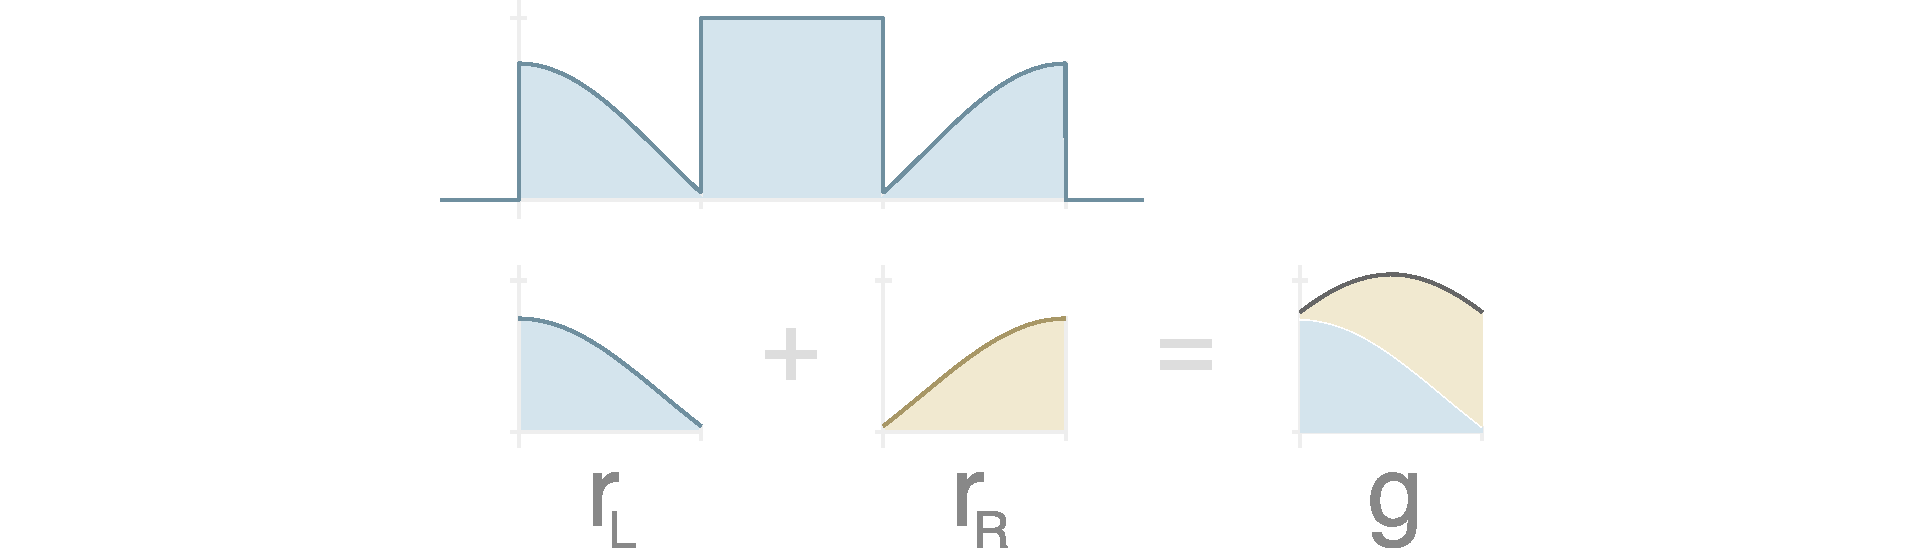
\includegraphics{images/pdfs/nonpl_setup.pdf}
\caption{An example showing how \(r_L\), \(r_R\), and \(g\) are
extracted from a function \(f\), shown on top.}\label{fig:nonpl_setup}
\end{figure}

I'll show that many copies of the shape of \(g\) must dominate the
landscape of \(f\) in order for it to be exactly self-replicating.

Now suppose that, in addition to having \(f(x)=0\) outside of \([0,3]\),
\(f\) is also exactly self-replicating. I'll use (\ref{eq:exact_defn})
to define functions \(f_L\), \(f_R\), and \(f_S\) in terms of \(f\) and
the functions \(s\), \(t_1\), and \(t_2\) from (\ref{eq:s_t1_t2}).
Notice that

\[\begin{array}{rcl}
\big(f_S \restrict [2,3]\big) & = & \big(f_L + f_R \restrict [2, 3]\big) \\
 & = & r_L + r_R = g. \\
\end{array}\]

Since \(f_L(x) = f_S(t_1(x))\), and \(t_1\) maps
\([1\tfrac{1}{3}, 1\tfrac{2}{3}]\) to \([2,3]\), this means
\((\,f=f_L \restrict [1\tfrac{1}{3}, 1\tfrac{2}{3}]) = g\). Below, I'll
show how repeated application of this kind of logic determines the
non-ramp values of \(f\) almost everywhere; a boolean property
\(P:\R\to\{\text{true},\text{false}\}\) is defined to be true
\href{https://en.wikipedia.org/wiki/Almost_everywhere}{\emph{almost
everywhere}} when the set \(\{x : P(x) = \text{false}\}\) has measure
zero.

\newcommand{\zerotwo}{\big\{\raise1.5pt\hbox{$\genfrac{}{}{0pt}{}
{\lower1.8pt\hbox{$\smash{\scriptstyle 0}$}}
{\lower1pt\hbox{$\smash{\scriptstyle 2}$}}$}\big\}}

\newcommand{\lstar}{\overline{*}_3}

At this point it will be useful to begin using base-3 notation for the
intervals at hand. If \(s\) is a finite string with digits from the set
\(\{0, 1, 2\}\), then let \(0.s\lstar\) denote the closure of the set of
points whose base-3 expansion begins with \(0.s\). For example,
\(0.11\lstar\) denotes the interval \([0.11_3, 0.12_3]\) while
\(0.12\lstar\) denotes the interval \([0.12_3, 0.20_3]\). I'll also use
\(\zerotwo\) to denote a digit that may be either a 0 or a 2; for
example, \(0.1\zerotwo 1\lstar\) denotes the union of intervals
\([0.101_3, 0.102_3]\) and \([0.121_3, 0.122_3]\).

Now, instead of writing
\((\,f \restrict [1\tfrac{1}{3}, 1\tfrac{2}{3}]) = g\), I can write

\begin{equation}\big(\,f \restrict 1.1\lstar\big) = g.\label{eq:nonpl_base_case}\end{equation}

It's possible to generalize this last equation so that it defines \(f\)
almost everywhere on the interval \([1, 2]\).

Recall that the notation \(1.\zerotwo^k1\lstar\) indicates a union of
closed intervals. In the next theorem, the notation
\((\,f \restrict \cup_i [a_i,b_i]) = g\) indicates that, for every \(i\)
in the union, \((\,f \restrict [a_i,b_i]) = g\).

\textbf{Theorem 1} \(\;\) \emph{Suppose that \(f\) is exactly
self-replicating with functions \(s,\) \(t_1,\) and \(t_2\) as given in
(\ref{eq:s_t1_t2}). Also suppose that \(f(x) = 0\) outside of \([0,3]\),
and that \(g\) is defined as in (\ref{eq:rL_rR_g}). Then, for any
\(k\ge 0\), \[\big(\,f \restrict 1.\zerotwo^k1\lstar\big)=g.\]}

\textbf{Proof} \(\;\) The proof is by induction on \(k\). Equation
(\ref{eq:nonpl_base_case}) provides the base case.

For the inductive step, suppose

\[\big(f=f_L \restrict 1.\zerotwo^k1\lstar \big) = g.\]

Then

\[\big(f_R \restrict 3 + 0.\zerotwo^k1\lstar \big) = g,\]

so that

\[\big(f_S \restrict \{1,3\} + 0.\zerotwo^k1\lstar \big) = g.\]

Apply \(t_1^{-1}\) to the domain set of \(f_S\) to determine the
corresponding domain set of \(f_L\):

\[\big(f \restrict 1.\zerotwo^{k+1}1\lstar \big) = g.\]

\hfill\(\Box\)

Define the sets \(G_k\) and \(G\) via

\begin{equation}G_k = 1.\zerotwo^k1\lstar \quad\text{and}\quad
  G = \cup_{k \ge 0}G_k.\label{eq:Gk_G}\end{equation}

Figure~\ref{fig:nonpl_process} illustrates \(G_k\) for low values of
\(k\).

\begin{figure}
\centering
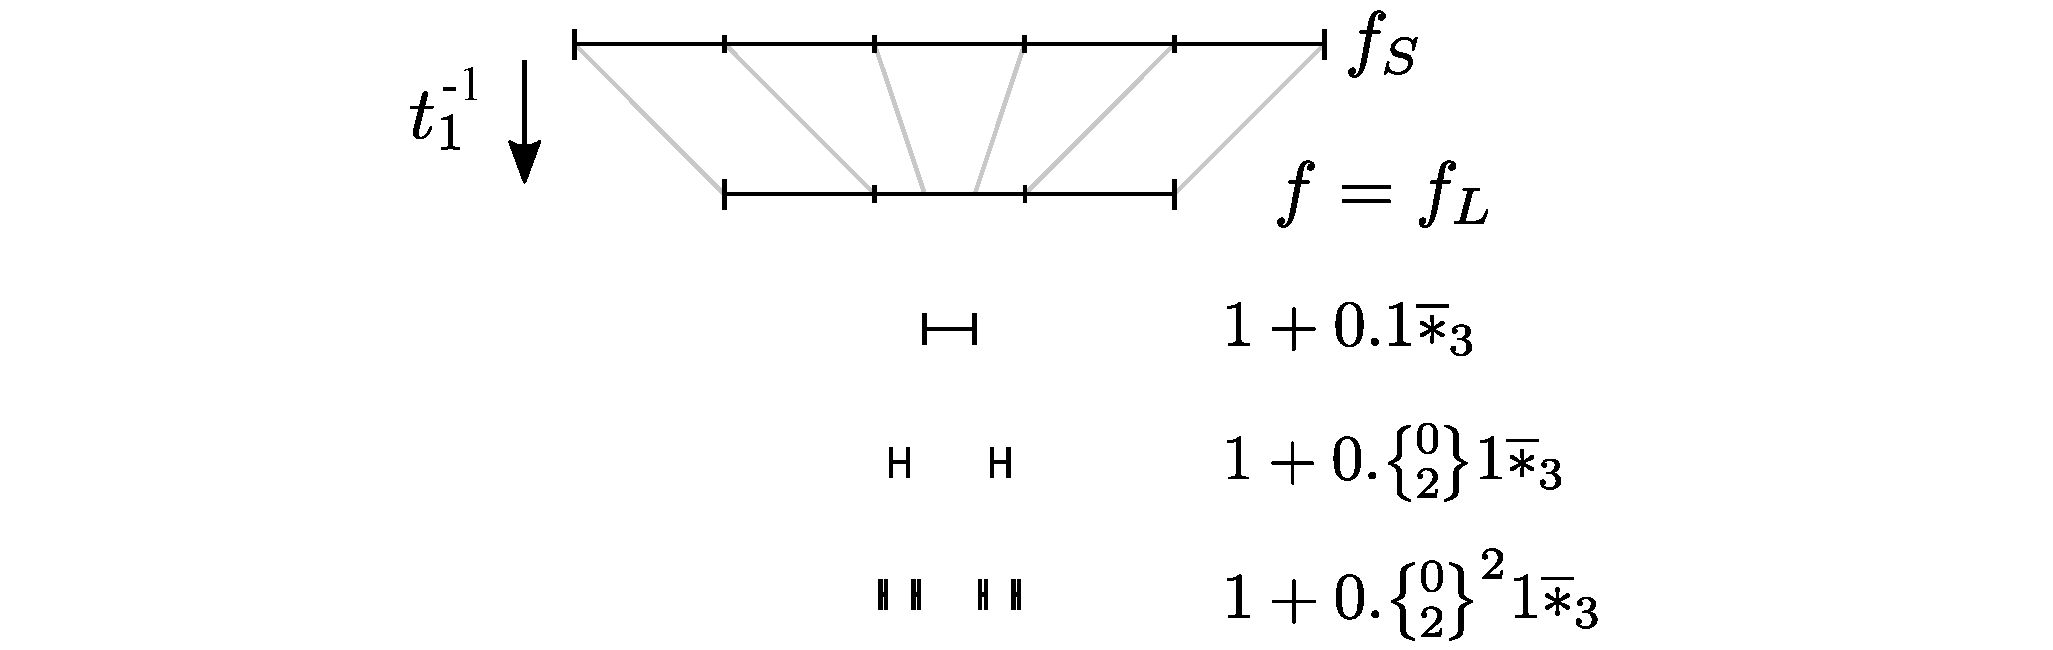
\includegraphics{images/pdfs/nonpl_process.pdf}
\caption{The inductive process in the proof of theorem 1. The top line
is the domain \([0,5]\) of \(\,f_S\); the line below that is the domain
\([0,3]\) of \(\,f;\) then the subsets of \([1,2]\) on which \(f\) is
described as the induction proceeds.}\label{fig:nonpl_process}
\end{figure}

Let's check that the sets \(G_k\) are disjoint. Suppose \(x_j\in G_j\)
and \(x_k\in G_k\), where \(j < k\), and we'll work with the standard
base-3 notation in which an all-2 tail is disallowed. Either
\(x_k=0.\zerotwo^k1\!\ldots\) or \(x_k=0.\zerotwo^k2\). There are two
similar cases for \(x_j\). In the first case, the \((j+1)^\text{th}\)
digit of \(x_j\) is 1, which is impossible for the \((j+1)\text{th}\)
digit of \(x_k\). In the second case, the \((j+1)^\text{th}\) digit of
\(x_j\) is 2 and all subsequent digits, including the
\((k+1)^\text{th}\), are 0; this excludes equality since the
\((k+1)^\text{th}\) digit \(x_k\) can't be 0. In either case,
\(x_j\ne x_k\), confirming that \(G_j\) and \(G_k\) are disjoint.

Using this disjointedness, we can find the total measure of their union
\(G\) as follows:

\[\mu(G) = \sum_{k \ge 0}\mu(G_k) = \sum_{k\ge 0}
\frac{1}{3}\left(\frac{2}{3}\right)^k = 1.\]

Since each \(G_k\subset [1,2]\), this justifies the claim that theorem 1
characterizes \(f\) almost everywhere in that interval.

\newcommand{\cantor}{\mathcal{C}}

Readers familiar with the
\href{https://en.wikipedia.org/wiki/Cantor_set}{\emph{Cantor set}}
\(\cantor\) may notice that it's closely related to the set \(G\). In
fact, \(\cantor\) is exactly the closure of \((1,2)-G\) shifted by a
unit to reside within \([0,1].\)

What values may \(f\) take on for the points \(x\in (1,2) - G\)? The
choice is still not arbitrary as the values remain related. I'll explore
this question next.

Given \(x\in (1,2)\), there is some \(k\) with \(x\in G_k\) iff the
base-3 expansion of \(x\) contains a 1 or if it ends with the tail
\(\overline{0}\). This can be expressed as:

\begin{equation}\begin{array}{l}
\text{For } x\in (1,2),\quad
  \Rule{0px}{1px}{0.7em}x\not\in G \;\;\Leftrightarrow\;\; \\
  x \in 1.\zerotwo^\infty_3 -\,
  \bigcup_{k\ge 0} 1.\zerotwo^k\overline{0}_3.
\end{array}\label{eq:onetwo_lessG}\end{equation}

From here on, I'll more formally use the word \emph{expansion} --- based
on the idea of the base-3 expansion of a number in \([0,1]\) --- to
indicate a function \(E:\mathbb{N}_{\ge 1}\to \{0, 1, 2\}\) which
denotes the value \(v(E) = \sum_{k\ge 1}E(k)/3^k.\) If \(x=v(E)\), we
may write \(x = 0.E_3\) and think of \(E\) as an infinite string on the
alphabet \(\{0,1,2\}\).

Suppose that \(f(x) = y\) for some \(x\in (1,2)\). Let \(E\) be the
expansion with \(x=1.E_3\); note that \(E\) cannot be the all-zero
string \(\overline 0\) nor the all-two string \(\overline 2\) since
\(x\in (1,2)\). Then \(f_S(x+\{0,2\}) = y\) and, by applying \(t_1\),
\(f(x') = y\) for both \(x' = (x+2)/3\) and \(x' = (x+4)/3\). In
expansion notation, we can write these last two equations as
\(x' = x/3 + 2/3 = 0.1E_3 + 0.2_3 = 1.0E_3\) and as
\(x' = x/3 + 4/3 = 0.1E_3 + 1.1_3 = 1.2E_3\). We can summarize this
reasoning as

\begin{equation}E\ne \overline 0, \overline 2 \optquad\Rightarrow\optquad
f(1.\zerotwo E_3) = f(1.E_3).\smallscrneg\label{eq:h_reln}\end{equation}

\newcommand{\tail}{\text{tail}}

We can expand on this idea to partition \((1,2) - G\) into subsets on
which \(f\) must have the same value. To do that, it will be useful to
define the \emph{tail} of an expansion as a way to capture end-of-string
behavior. More precisely, if \(E\) is an expansion, then define
\(\tail(E)\) via

\[\bigscr{\tail(E) = \big\{\text{expansion }\eta \;\big|\;
\exists\, j, k: 
E(j + m) = \eta(k + m) \,\forall\, m \ge 0\big\}.}
\smallscr{\begin{array}{l}\tail(E) = \big\{\text{expansion }\eta \;\big|\;
\exists\, j, k: \\
\quad E(j + m) = \eta(k + m) \,\forall\, m \ge 0\big\}.\end{array}}\]

Intuitively, \(\tail(E)\) is the set of all numbers in \([0, 1]\) with
the same final sequence of base-3 digits as \(E\), ignoring any finite
prefix of either expansion. For example, \(x=0.21021\overline{011}_3\)
and \(y=0.001\overline{011}_3\) have
\(\text{tail}(x) = \text{tail}(y)\).

The following theorem builds on equation (\ref{eq:h_reln}).

\textbf{Theorem 2} \(\;\) \emph{Suppose that \(f\) is exactly
self-replicating with functions \(s,\) \(t_1,\) and \(t_2\) as given in
(\ref{eq:s_t1_t2}). Also suppose that \(G\) is defined as in
(\ref{eq:Gk_G}). Then, for} \(x,y\in (1,2)-G,\)

\[\tail(x) = \tail(y) \quad\Rightarrow\quad f(x) = f(y).\]

\textbf{Proof} \(\;\) Note that, by (\ref{eq:onetwo_lessG}), \(x\) and
\(y\) can be expressed in expansion notation as \(x=1.E_3\) and
\(y=1.F_3\) where both \(E\) and \(F\) exclude 1 from their range, and
neither has an all-0 tail.

Since \(\tail(x) = \tail(y)\), then there exist integers \(j, k\) such
that

\begin{equation}E(j+m)=F(k+m)\; \forall m\ge 0.\label{eq:thm2_pf}\end{equation}

Let \(p_E\) be the length-\(j\) prefix of \(E\) and \(p_F\) be the
length-\(k\) prefix of \(F\), and choose the expansions \(E'\) and
\(F'\) so that

\[
\bigscr{
x = 1.E_3 = 1.p_EE'_3 \quad\text{ and }\quad y = 1.F_3 = 1.p_FF'_3.
}
\smallscr{
\begin{array}{rcl}
x & = & 1.E_3 = 1.p_EE'_3 \quad\text{ and }\\
y & = & 1.F_3 = 1.p_FF'_3.
\end{array}
}
\]

By (\ref{eq:thm2_pf}), \(E'=F'\). By repeated application of
(\ref{eq:h_reln}), \(f(1.p_EE'_3) = f(1.E'_3)\) and
\(f(1.p_FF'_3) = f(1.F'_3)\). The final result is that

\[f(x) = f(1.E'_3) = f(1.F'_3) = f(y).\]

\hfill\(\Box\)

It turns out that theorems 1 and 2 capture \emph{all} of the
restrictions needed for \(f\) to be exactly self-replicating. This idea
is formalized by the next theorem.

\textbf{Theorem 3} \(\;\) \emph{Suppose that \(f:\R\to\R\) has the value
0 outside the domain \([0, 3].\) Also suppose we're working in the
context of the functions \(s,\) \(t_1,\) and \(t_2\) as defined in
(\ref{eq:s_t1_t2}), and that the function \(g\) is defined as in
(\ref{eq:rL_rR_g}). Then \(f\) is exactly self-replicating iff}

\begin{equation}\eqnset{\begin{array}{lcll}
f(1.\zerotwo E_3) & \smallscrskip{-1em} = & \smallscrskip{-0.5em} f(1.E_3) & E\ne\overline 0,\overline 2;                \smallscrneg \\
f(1.1E_3)         & \smallscrskip{-1em} = & \smallscrskip{-0.5em} g(0.E_3) & \text{for any }E. \latexonlyrule{0pt}{14pt} \smallscrneg \\
\end{array} } \smallscrneg\label{eq:thm3}\end{equation}

\textbf{Proof} \(\;\) The forward direction --- that (\ref{eq:thm3}) is
a consequence of \(f\) being exactly self-replicating --- has already
been justified by (\ref{eq:nonpl_base_case}) and (\ref{eq:h_reln}). Note
that these last two equations are each expanded upon in theorems 1 and
2.

To verify the other direction, it will suffice to show that, if
(\ref{eq:thm3}) is true, then so is:

\begin{equation}f(x) = f_S(t_1(x));\label{eq:thm3_pf}\end{equation}

this equation is enough to ensure that the definition of an exactly
self-replicating function, given by (\ref{eq:exact_defn}), is satisfied.

Suppose \(x=1.CE_3 \in (1,2)\), where \(C \in \{0, 1, 2\}\) and \(E\)
does not have an all-2 tail; let \(x' = t_1(x)\). The argument can be
split into three cases based on the value of \(C\).

\emph{Case} \(C=0:\;\) In this case, \(x' = 1.E_3 \in (1, 2)\) and
\(f_S(x') = f(x') = f(1.E_3).\) Apply (\ref{eq:thm3}) to see that
\(f(1.E_3) = f(1.0E_3) = f(x)\), verifying (\ref{eq:thm3_pf}).

\emph{Case} \(C=1:\;\) In this case, \(x' = 2.E_3 \in [2,3].\) So
\(f_S(x') = f(2.E_3) + f(0.E_3) =\) \(r_R(0.E_3) + r_L(0.E_3) =\)
\(g(0.E_3).\) Apply (\ref{eq:thm3}) and continue:
\(g(0.E_3) = f(1.1E_3) = f(x).\) This also verifies (\ref{eq:thm3_pf}).

\emph{Case} \(C=2:\;\) This cases is similar to \(C=0,\) except that
\(x' \in (3,4).\) Specifically, \(f_S(x') = f(x'-2) =\) \(f(1.E_3) =\)
\(f(1.2E_3) = f(x),\) again verifying (\ref{eq:thm3_pf}).

In all cases, equation (\ref{eq:thm3_pf}) holds, ensuring that \(f\) is
indeed exactly self-replicating.

\hfill\(\Box\)

Call the function \(h\) \emph{tail-consistent} on a domain set \(A\) iff
\(\tail(x) = \tail(y) \;\Rightarrow\;\) \(h(x) = h(y)\) for any
\(x,y \in A.\) There's a bijection between the exactly self-replicating
functions characterized by theorem 3 and an arbitrary choice of the
following three functions:

\[\begin{array}{ll}
r_L : [0,1] \to \R, \\
r_R : [0,1] \to \R, & \text{and} \\
h   : (1,2) - G \to \R & \text{which is tail-consistent.}
\end{array}\]

Any choice of these three functions results in an exactly
self-replicating function. Given any exactly self-replicating function
\(f\) with respect to \(s,\) \(t_1,\) and \(t_2\) given in
(\ref{eq:s_t1_t2}), and with \(f(x) = 0\) outside \([0,3]\), there
exists a unique corresponding triple \(r_L,\) \(r_R,\) and \(h\).
Theorem 3 is the key to verifying that this correspondence between such
\(f\) and triples \((r_L, r_R, h)\) is indeed a bijection.

Below is an example image depicting the function we get by choosing
\(r_L(x) = \cos(2x)/2 + 1/4\) and \(r_R(x) = r_L(1-x)\). The \(h\)
function has the constant value \(r_L(0) + r_R(0)\).

\begin{figure}
\centering
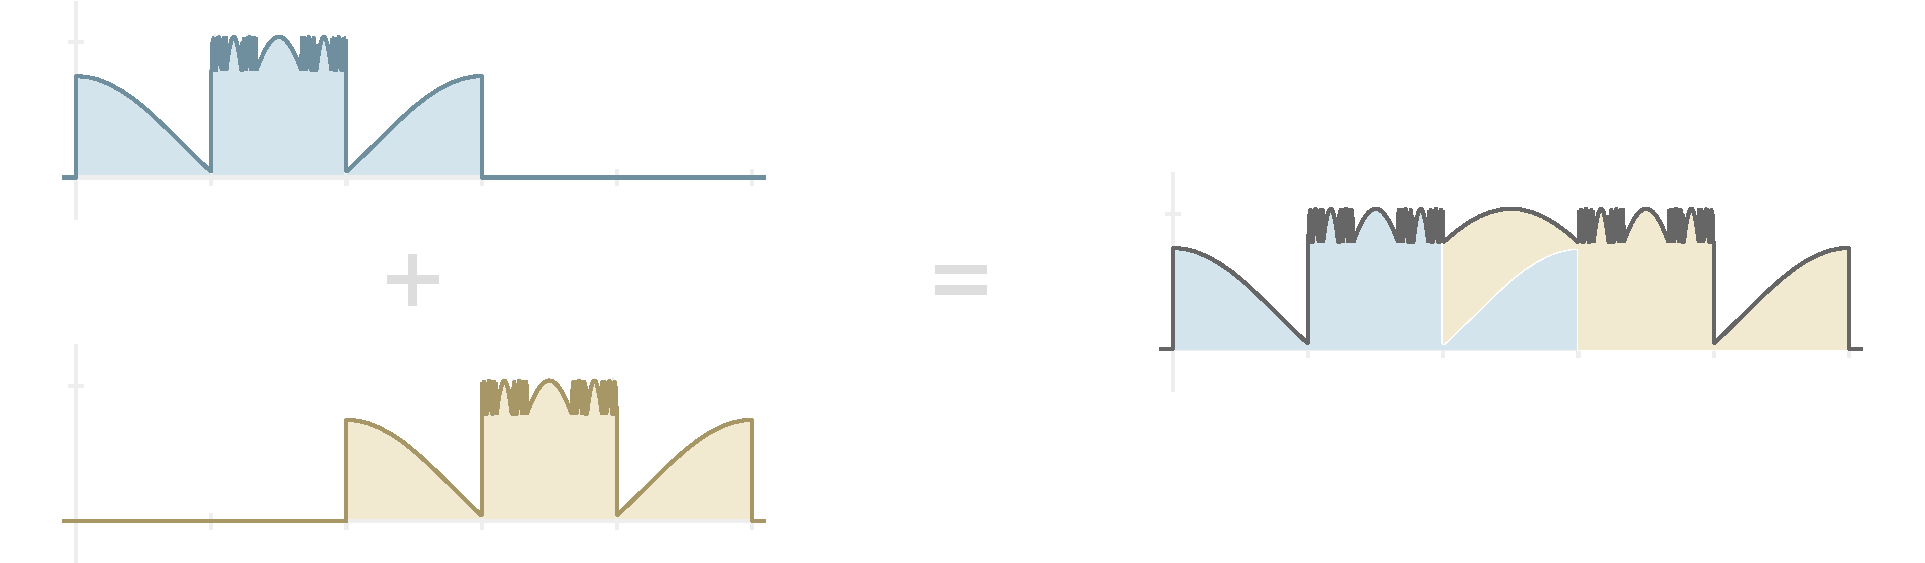
\includegraphics{images/pdfs/nonplateau.pdf}
\caption{An exactly self-replicating function \(f\) completely
determined by \(r_L(x) = \cos(2x)/2 + 1/4\), \(r_R(x) = r_L(1 - x)\),
and the value \(f(x) = r_L(0) + r_R(0)\) for all \(x\) not determined by
\(r_L\) and \(r_R\).}\label{fig:nonplateau}
\end{figure}

Next I'll examine a famous function which is \emph{not} exactly
self-replicating, but which can be seen as approximately
self-replicating: the normal curve.

\section*{References}\label{references}
\addcontentsline{toc}{section}{References}

\hypertarget{refs}{}
\hypertarget{ref-taocp1}{}
Knuth, Donald E. 1998. \emph{Fundamental Algorithms}. Third Ed. Vol. 1.
The Art of Computer Programming. Addison-Wesley.

\end{document}
